\chapter{A brief history of data science}
\label{chap:history}

There are many points of view regarding the origin of data science.  For the sake of
contextualization, I separate the topic into two approaches: the history of the term itself
and a broad timeline of data-driven sciences, highlighting the important figures in each
age.

I believe that the history of the term is important for understanding the context of the
discipline. Over the years, the term has been employed to label quite different fields of
study.  Before presenting my view on the term, I present the views of two influential
figures in the history of data science: Peter Naur and William Cleveland.

Moreover, studying the key facts and figures in the history of data-driven sciences
enables us to comprehend the evolution of the field and hopefully guide us towards evolving it
further.  Besides, history also teaches us ways to avoid repeating the same mistakes.

Most of the significant theories and methods in data science have been developed
simultaneously across different fields, such as statistics, computer science, and engineering.
The history of data-driven sciences is long and rich. I present a timeline of the ages of
data handling and the most important milestones of data analysis.

I do not intend to provide a comprehensive history of data science.  I aim to provide
enough context to support the development of the material in the following chapters,
sometimes avoiding directions that are not relevant in the context of inductive learning.

\section{The term ``data science''}

The term data science is relatively recent and has been used to label rather different fields of
study.  In the following, I emphasize the history of a few notable usages of the term.

\def\naurds{(0,0) circle (20mm)}
\def\naurcs{(0:5mm) circle (15mm)}
\def\naurde{(0:40mm) circle (15mm)}

\colorlet{circle edge}{black!50}
\colorlet{circle area}{black!20}

\tikzset{filled/.style={fill=circle area, draw=circle edge, thick},
    outline/.style={draw=circle edge, thick}}

\paragraph{Peter Naur (1928 -- 2016)}

The term ``data science'' itself was coined in the 1960s by Peter Naur. Naur was
a Danish computer scientist and mathematician who made significant contributions to the
field of computer science, including his work on the development of programming
languages\footnote{He is best remembered as a contributor, with John Backus, to the
\gls{bnf} notation used in describing the syntax for most programming
languages.}.
His ideas and concepts laid the groundwork for the way we think about programming and data
processing today.

Naur disliked the term computer science and suggested it be called datalogy or data
science.  In the 1960s, the subject was practised in Denmark under Peter
Naur's term datalogy, which means the science of data and data processes.

He coined this term to emphasize the importance of data as a fundamental component of
computer science and to encourage a broader perspective on the field that included
data-related aspects. At that time, the field was primarily centered on programming
techniques, but Naur's concept broadened the scope to recognize the intrinsic role of data
in computation.

In his book\footfullcite{Naur1974}, ``Concise Survey of Computer Methods'', he
parts from the concept that \emph{data} is ``a representation of facts or ideas in a
formalised manner capable of being communicated or manipulated by some
process.''\footnote{I. H. Gould (ed.): ‘IFIP guide to concepts and terms in data
processing’, North-Holland Publ. Co., Amsterdam, 1971.} Note however that his view of the
science only ``deals with data [\dots] while the relation of data to what they represent
is delegated to other fields and sciences.''

\begin{figure}
  \centering
  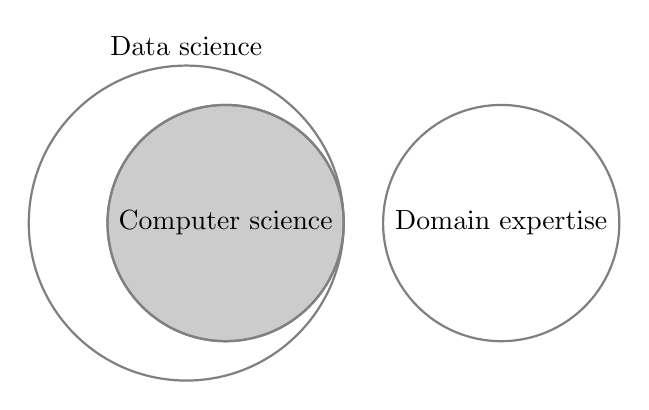
\begin{tikzpicture}
    \begin{scope}
      \clip \naurds;
      \fill[filled] \naurcs;
    \end{scope}
    \draw[outline] \naurds node(ds) {};
    \draw[outline] \naurcs node {Computer science};
    \draw[outline] \naurde node {Domain expertise};
    \node[anchor=north,above] at (0,2) {Data science};
  \end{tikzpicture}
  \caption{
    Naur's view of data science.
    For Naur, data science studies the techniques to deal
    with data, but he delegates the meaning of data to other fields.
  }
  \label{fig:naur}
\end{figure}

It is interesting to see the central role he gave to data in the field of computer
science. His view that the relation of data to what they represent is delegated to other
fields and sciences is still debatable today.  Some scientists argue that data science
should focus on the techniques to deal with data, while others argue that data science
should encompass the whole business domain.  A depiction of Naur's view of data science is
shown in \cref{fig:naur}.

\def\clevelandds{(0,0) circle (20mm)}
\def\clevelandst{(0:-5mm) circle (15mm)}
\def\clevelandde {(2,1) circle (15mm)}
\def\clevelandcs {(2,-1) circle (15mm)}

\paragraph{William Cleveland (born 1943)}

In 2001, a prominent statistician used the term ``data science'' in his work to describe a
new discipline that comes from his ``plan to enlarge the major areas of technical work of
the field of statistics\footfullcite{Cleveland2001}.''
In 2014, that work was republished\footnote{W. S. Cleveland.
Data Science: An Action Plan for the Field of Statistics. Statistical Analysis and Data
Mining, 7:414–417, 2014. reprinting of 2001 article in ISI Review, Vol 69.}.
He advocates the expansion of statistics beyond theory into technical areas, significantly
changing statistics.  Thus, it warranted a new name.

As a result, William Swain Cleveland II is credited with defining data science as it is most
used today. He is a highly influential figure in the fields of statistics, machine
learning, data visualization, data analysis for multidisciplinary studies, and high
performance computing for deep data analysis.

\begin{figure}
  \centering
  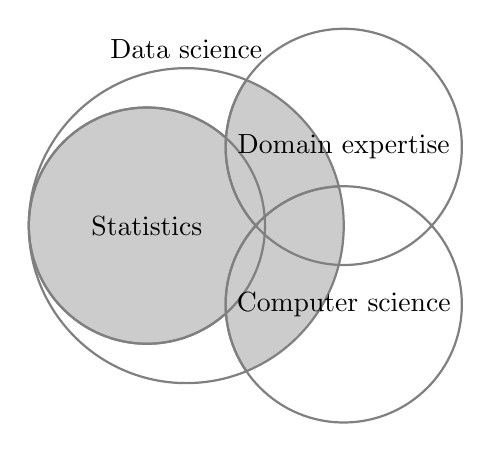
\begin{tikzpicture}
    \begin{scope}
      \clip \clevelandds;
      \fill[filled] \clevelandst;
      \fill[filled] \clevelandde;
      \fill[filled] \clevelandcs;
    \end{scope}
    \draw[outline] \clevelandds node(ds) {};
    \draw[outline] \clevelandst node {Statistics};
    \draw[outline] \clevelandde node {Domain expertise};
    \draw[outline] \clevelandcs node {Computer science};
    \node[anchor=north,above] at (0,2) {Data science};
  \end{tikzpicture}
  \caption{
    Cleveland's view of data science.
    For Cleveland, data science is the ``modern'' statistics,
    where it is enlarged by computer science and domain expertise.
  }
  \label{fig:cleveland}
\end{figure}

In his view, data science is the ``modern'' statistics, where it is enlarged by computer
science methods and domain expertise.  An illustration of Cleveland's view of data science
is shown in \cref{fig:cleveland}.  It is important to note that Cleveland never defined an
explicit list of computer science fields and business domains that should be included in
the new discipline.  The main idea is that statistics should rely on computational methods
and that the domain expertise should be considered in the analysis.

\paragraph{Buzzword or a new science?}

Be aware that scientific literature has no consensus on the definition of data science, and it is still considered
by some to be a buzzword\footnote{Press, Gil. ``Data Science: What's The Half-Life of a
Buzzword?''. Forbes. Available at
\href{https://www.forbes.com/sites/gilpress/2013/08/19/data-science-whats-the-half-life-of-a-buzzword/}%
  {forbes.com/sites/gilpress/2013/08/19/data-science-whats-the-half-life-of-a-buzzword}.}.

Most of the usages of the term in literature and in the media are either a rough
reference to a set of data-driven techniques or a marketing strategy.  Naur
(\cref{fig:naur}) and Cleveland (\cref{fig:cleveland}) are among the few that try to
carefully define the term.  However, both of them do not see data science as an
independent field of study, but rather an enlarged scope of an existing science.  I disagree;
the social and economic demand for data-driven solutions has led to an evolution in our
understanding of the challenges we are facing.  As a result, we see many ``data
scientists'' being hired and many ``data science degree'' programs emerging.

In \cref{chap:data}, I dare to provide a (yet another) definition for the term.  I
argue that its object of study can be precisely established to support it as a new
science.

\section{Timeline and historical markers}

\textcite{Kelleher2018}\footfullcite{Kelleher2018} provides an interesting timeline of data-driven methods and
influential figures in the field.  I reproduce it here with some changes, including
some omissions and additions.  On the subject of data analysis, I include some
exceptional remarks
from \textcite{Vapnik1999b}\footfullcite{Vapnik1999b}.

I first address data handling --- which includes data sources, collection, organization,
storage, and transformation ---, and then data analysis and knowledge extraction.

\subsection{Timeline of data handling}
\label{sub:time-handling}

The importance of collecting and organizing data goes without saying.  Data fuels analysis and
decision making.  In the following, I present some of the most important milestones in the history
of data handling.

\begin{figure}
  \centering
  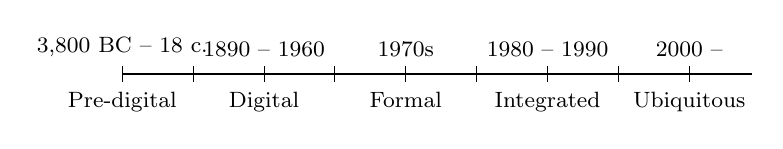
\begin{tikzpicture}
    \draw (0,0) -- (8,0);
    \foreach \x in {0,1,...,8} {
      \draw (0.9 * \x,-0.1) -- (0.9 * \x,0.1);
    }
    \foreach \x/\y/\z in {%
        0/Pre-digital/{3,800 BC -- \nth{18} c.},
        2/Digital/{1890 -- 1960},
        4/Formal/{1970s},
        6/Integrated/{1980 -- 1990},
        8/Ubiquitous/{2000 --}} {
      \node[anchor=north] at (0.9 * \x,-0.1) {\footnotesize\y};
      \node[anchor=south] at (0.9 * \x,0.1) {\footnotesize\z};
    }
  \end{tikzpicture}
  \caption{Timeline of the ages of data handling.}
  \label{fig:data-handling-history}
\end{figure}

\Cref{fig:data-handling-history} illustrates the proposed timeline.  Ages have no absolute
boundaries, but rather periods where some important events happened.  Also, observe that
the timescale is not linear.  The Pre-digital Age is the longest period, and one could
divide it into smaller periods.  My choices of ages and their boundaries are motivated by
didactic reasons.

\subsubsection{Pre-digital age}

We can consider the earliest records of data collection to be the notches on sticks and
bones (probably) used to keep track of the passing of time.  The Lebombo bone, a baboon fibula with
notches, is one of the earliest known mathematical objects.  It was found in the Lebombo
Mountains located between South Africa and Eswatini.
They estimate it is more
than 40,000 years old. It is conjectured to be a tally stick, but its exact purpose is
unknown. Its 29 notches suggest that it may have been used as a lunar phase counter.
However, since it is broken at one end, the 29 notches may or may not be the total
number\footfullcite{Beaumont2013}.

Another milestone in the history of data collection is the record of
demographic data.  One of the first known censuses was conducted in 3,800 BC in the Babylonian
Empire.  It was ordered to assess the population and resources of
the empire.  Records were stored on clay tiles\footfullcite{Grajalez2013}.

Since the early forms of writing, humanity's abilities to register data and events
increased significantly.  The first known written records date back to around 3,500 BC, the
Sumerian archaic (pre-cuneiform) writing.  This writing system was used to represent
commodities using clay tokens and to record transactions\footfullcite{Ifrah1998}.

``Data storage'' was also a challenge.  Some important devices that increased our capacity
to register textual information are the Sumerian clay tablets (3,500 BC), the Egyptian
papyrus (3,000 BC), the Roman wax tablets (100 BC), the codex
(100 AD), the Chinese paper (200 AD), the printing press (1440), and the typewriter (1868).

% Talvez citar na parte de análise de dados
% Other mechanisms were also developed to store information in a more structured way.  Some
% important devices are
% the abacus (2,700 BC), the Antikythera mechanism (150 -- 100 BC), the
% Chinese South Pointing Chariot (260 AD), the Pascaline (1642), the Jacquard loom (1801),
% the Babbage Difference Engine (1822), the Babbage Analytical Engine (1837).

Besides those improvements in unstructured data storage, at least in the Western and
Middle Eastern world, there are no significant advances in structured data collection
until the \nth{19} century.  (An Eastern timeline research seems much harder to perform.
Unfortunately, I left it out in this book.)

I consider a major influential figure in the history of data
collection to be Florence Nightingale (1820 -- 1910).  She was a passionate statistician
and probably the first person to use statistics to influence public and official
opinion.  The meticulous records she kept during the Crimean War
(1853 -- 1856) were the evidence that saved lives --- part of the mortality came from lack
of sanitation.  She was also the first to use
statistical graphics to present data in a way that was easy to understand.  She is
credited with developing a form of the pie chart now known as the polar area
diagram.  She also reformed healthcare in the United Kingdom and
is considered the founder of modern nursing; where a great part of the work was to collect
data in a standardized way to quickly draw conclusions\footfullcite{Grajalez2013}.

\subsubsection{Digital age}

In the modern period, several devices were developed to store digital\footnote{Digital
means the representation of information in (finite) discrete form.  The term comes from the Latin
digitus, meaning finger, because it is the natural way to count using fingers.  Digital
here does not mean electronic.}
information.  One particular device that is important for data collection is the punched
card.  It is a piece of stiff paper that contains digital information represented by the
presence or absence of holes in predefined positions.  The information can be read by a
mechanical or electrical device called a card reader.  The earliest famous usage of
punched cards was by Basile Bouchon (1725) to control looms.  Most of the advances until
the 1880s were about the automation of machines (data processing) using hand-punched cards, and not
particularly specialized for data collection.

However, the 1890 census in the United States was the first to use machine-readable
punched cards to tabulate data. Processing 1880 census data took eight years, so the
Census Bureau contracted Herman Hollerith (1860 -- 1929) to design and build a tabulating
machine.  He founded the Tabulating Machine Company in 1896, which later merged with other
companies to become \gls{ibm} in 1924. Later
models of the tabulating machine were widely used for business applications such as
accounting and inventory control. Punched card technology remained a prevalent method of
data processing for several decades until more advanced electronic computers were
developed in the mid-\nth{20} century.

The invention of the digital computer is responsible for a revolution in data handling.
The amount of information we can capture and store increased exponentially.  ENIAC (1945) was
the first electronic general-purpose computer.  It was Turing-complete, digital, and
capable of being reprogrammed to solve a full range of computing problems.
It had 20 words of internal memory, each capable of storing a 10-digit decimal integer number.
Programs and data were entered by setting switches and inserting punched cards.

For the 1950 census, the United States Census Bureau used the
UNIVAC I (Universal Automatic Computer I), the first commercially produced computer in the
United States\footnote{Read more in \url{https://www.census.gov/history/www/innovations/}.}.

It goes without saying that digital computers have become much more powerful and
sophisticated since then.  The data collection process has been easily automated and
scaled to a level that was unimaginable before.  However, ``where'' storing data is
not the only challenge.  ``How'' to store data is also a challenge.  The next period of
history addresses this issue.

\subsubsection{Formal age}

In 1970, Edgar Frank Codd (1923 -- 2003), a British computer scientist,
published a paper entitled ``A Relational Model
of Data for Large Shared Data Banks''\footfullcite{Codd1970}.  In this paper, he introduced
the concept of a relational model for database management.

A relational model organizes data in tables (relations) where each row represents a record
and each column represents an attribute of the record.  The tables are related by common
fields.  Codd showed means to organize the tables of a relational database to minimize
data redundancy and improve data integrity.  \Cref{sec:normalization} provides more details
on the topic.

His work was a breakthrough in the field of data management.  The standardization of
relational databases led to the development of \gls{sql} in 1974.
SQL is a domain-specific language used in programming and designed for managing data held
in a \gls{rdbms}.

As a result, a new challenge rapidly emerged: how to aggregate data from different
sources. Once data is stored in a relational database, it is easy to query and manage
it. However, data is usually stored in different databases, and it is not always possible
to directly combine them.

\subsubsection{Integrated age}

The solution to this problem was the development of the \gls{etl}
process.  \gls{etl} is a process in data warehousing responsible for extracting data from
several sources, transforming it into a format that can be analyzed, and loading it into a
data warehouse.

The concept of data warehousing dates back to the late 1980s when IBM researchers Barry
Devlin and Paul Murphy developed the ``business data warehouse.''

Two major figures in the history of \gls{etl} are Ralph Kimball (born 1944) and Bill Inmon (born
1945), both American computer scientists.  Although they
differ in their approaches, they both agree that data warehousing is the foundation for
\gls{bi} and analytics, and that data warehouses should be designed to
be easy to understand and fast to query for business users.

A famous debate between Kimball and Inmon is the top-down versus bottom-up approach to
data warehousing.  Inmon's approach is top-down, where the data warehouse is designed
first and then the data marts\footnote{A data mart is a specialized subset of a data
warehouse that is designed to serve the needs of a specific business unit, department, or
functional area within an organization.} are created from the data warehouse.  Kimball's
approach is bottom-up, where the data marts are created first and then the data warehouse
is created from the data marts.

One of the earliest and most famous case studies of the implementation of a data warehouse
is that of Walmart. In the early 1990s, Walmart faced the challenge of managing and
analyzing vast amounts of data from its stores across the United States. The company
needed a solution that would enable comprehensive reporting and analysis to support
decision-making processes.  The solution was to implement a data warehouse that would
integrate data from various sources and provide a single source of truth for the
organization.

\subsubsection{Ubiquitous age}

The last and current period of history is the ubiquitous age.  It is characterized by the
proliferation of data sources.

The ubiquity of data generation and the evolution of data-centric technologies have been
made possible by a multitude of figures across various domains.

\begin{itemize}
  \itemsep0em
  \item Vinton Gray Cerf (born 1943) and Robert Elliot Kahn (born 1938), often referred to
    as the ``Fathers of the Internet,'' developed the TCP/IP protocols, which are
    fundamental to internet communication.
  \item Tim Berners-Lee (born 1955), credited with inventing the World Wide Web, laid the
    foundation for the massive data flow on the internet.
  \item Steven Paul Jobs (1955 -- 2011) and Stephen Wozniak (born 1950), from Apple Inc.,
    and William Henry Gates III (born 1955), from Microsoft Corporation, were responsible
    for the introduction of personal computers, leading to the democratization of data
    generation.
  \item Lawrence Edward Page (born 1973) and Sergey Mikhailovich Brin (born 1973), the
    founders of Google, transformed how we access and search for information.
  \item Mark Elliot Zuckerberg (born 1984), the co-founder of Facebook, played a crucial
    role in the rise of social media and the generation of vast amounts of user-generated
    content.
\end{itemize}

In terms of data handling, this change of landscape has brought about the
development of new technologies and techniques for data storage and processing.  Especially
the development of NoSQL databases and distributed computing frameworks.

NoSQL databases are non-relational databases that can store and process large volumes of
unstructured, semi-structured, and structured data.  They are highly scalable and
flexible, making them ideal for big data applications.

Some authors argue that the rise of big data is characterized by the five V's of big data:
Volume, Velocity, Variety, Veracity, and Value.  The amount of data generated is massive,
the speed at which data is generated is high, the types of data generated are diverse, the
quality of data generated is questionable, and the value of data generated is high.

Once massive amounts of unstructured data became available, the need for new data
processing techniques arose.  The development of distributed computing frameworks such as
Apache Hadoop and Apache Spark enabled the processing of massive amounts of data in a
distributed manner.

Douglass Read Cutting and Michael Cafarella, the developers of the software Apache Hadoop,
proposed both the \gls{hdfs} and MapReduce, which are the
cornerstones of the Hadoop framework, in 2006.  Hadoop's distributed storage and
processing capabilities enabled organizations to handle and analyze massive volumes of
data.

Currently, Google holds a patent for
MapReduce\footfullcite{Dean2008}.
However, their framework inherits from the architecture proposed in
\textcite{Hillis1985}\footfullcite{Hillis1985} thesis.
MapReduce is not particularly novel, but its simplicity and scalability made it popular.

Nowadays, another important topic is \gls{iot}.  IoT is a system of
interrelated computing devices that communicate with each other over the internet.
The devices can be anything from cellphones, coffee makers, washing machines, headphones,
lamps, wearable devices, and almost anything else you can think of.  The reality of IoT increased the
challenges of data handling, especially in terms of data storage and processing.

In summary, we currently live in a world where data is ubiquitous and comes in many
different forms.  The challenge is to collect, store, and process this data in a way that
is meaningful and useful, also respecting privacy and security.

\subsection{Timeline of data analysis}
\label{sub:time-analysis}

The way we think about data and knowledge extraction has evolved significantly over the
years.  In the following, I present some of the most important milestones in the history
of data analysis and knowledge extraction.

\begin{figure}
  \centering
  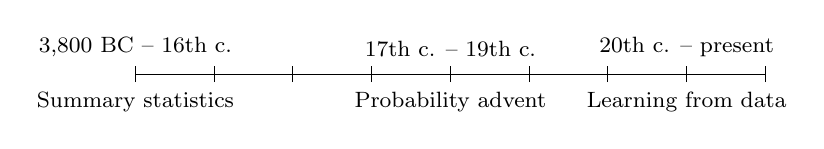
\begin{tikzpicture}
    \draw (0,0) -- (8,0);
    \foreach \x in {0,1,...,8} {
      \draw (\x,-0.1) -- (\x,0.1);
    }
    \foreach \x/\y/\z in {%
        0/Summary statistics/{3,800 BC -- 16th c.},
        4/Probability advent/{17th c. -- 19th c.},
        7/Learning from data/{20th c. -- present}} {
      \node[anchor=north] at (\x,-0.1) {\footnotesize\y};
      \node[anchor=south] at (\x,0.1) {\footnotesize\z};
    }
  \end{tikzpicture}
  \caption{Timeline of the ages of data analysis.}
  \label{fig:data-analysis-history}
\end{figure}

\Cref{fig:data-analysis-history} illustrates the proposed timeline.  I consider changes of
ages to be smooth transitions, and not strict boundaries.  The theoretical advances are
slower than the technological ones --- the latter influences more data handling than data
analysis ---, so not much has changed since the beginning of the \nth{20} century.

\subsubsection{Summary statistics}

The earliest known records of systematic data analysis date back to the first censuses.
The term \emph{statistics} itself refers to the analysis of data \emph{about the state},
including demographics and economics.  That early (and simplest) form of statistical
analysis is called \emph{summary statistics}, which consists of describing data in terms
of its central tendencies (e.g., arithmetic mean) and variability (e.g., range).

\subsubsection{Probability advent}

However, after the \nth{17} century, the foundations of modern probability theory were
laid out.  Important figures for developing that theory are Blaise Pascal (1623
-- 1662), Pierre de Fermat (1601 -- 1665), Christiaan Huygens (1629 -- 1695), and Jacob
Bernoulli (1655 -- 1705).

The foundation methods brought to life the field of statistical inference. In the
following years, important results were achieved.

\paragraph{Bayes' rule}

Reverend Thomas Bayes (1701 -- 1761) was an English statistician, philosopher, and
Presbyterian minister.  He is known for formulating a specific case of the theorem that
bears his name: Bayes' theorem.  The theorem is used to calculate conditional
probabilities using an algorithm (his Proposition 9, published in 1763) that uses evidence to calculate
limits on an unknown parameter.

The Bayes' rule is the foundation of learning from evidence, once it allows us to
calculate the probability of an event based on prior knowledge of conditions that might be
related to the event.  Classifiers based on Naïve Bayes --- the application of Bayes'
theorem with strong independence assumptions between known variables --- are likely to have
been used since the second half of the eighteenth century.

\paragraph{Gauss' method of least squares}

Johann Carl Friedrich Gauss (1777 -- 1855) was a German mathematician and physicist who made
significant contributions to many fields in mathematics and sciences.  Circa 1794, he
developed the method of least squares for calculating the orbit of Ceres to minimize the
impact of measurement error\footnote{The method was first published by Adrien-Marie
Legendre (1752 -- 1833) in 1805, but Gauss claimed in 1809 that he
had been using it since circa 1794.}.

The method of least squares marked the beginning of the field of regression analysis.  It
marked a shift to find the solution of systems of equations --- especially, overdetermined
systems --- using data instead of theoretical models.

\paragraph{Playfair's data visualization}

Another change in the way we analyze data was the development of data visualization.  Data
visualization is the graphical representation of information and data.

William Playfair (1759 -- 1823) was a secret agent on behalf of Great Britain during its
war with France in the 1790s.  He invented several types of diagrams between the 1780s and
1800s, such as the line, area, and bar chart of economic data, and the pie chart and circle
graph to show proportions.

\subsubsection{Learning from data}

In the twentieth century and beyond, new advances were made in the field of statistics.
The development of learning machines enabled the development of new techniques for data
analysis.

The recent advances in computation and data storage are crucial for the large-scale
application of these techniques.

This era is characterized by a change of focus from trying to fit data to a theoretical
model to trying to extract knowledge from data.  The main goal is to develop algorithms
that can learn from data with minimal human intervention.

\paragraph{Fisher's discriminant analysis}

In the 1930s, Sir Ronald A. Fisher (1890 -- 1962), a British polymath, developed
discriminant analysis\footnote{\url{https://digital.library.adelaide.edu.au/dspace/bitstream/2440/15227/1/138.pdf}},
which was initially used to find linear functions to solve the problem of separating two or
more classes of objects\footnote{After Rosenblatt's work, however, it was used to solve
inductive inference (classification) as well.  For curiosity, Fisher's paper
introduced the famous Iris data set.}.

The method is based on the so-called Fisher discriminant, which is a linear
combination of variables.  The method can be used not only for classification but also for
dimensionality reduction.

Tackling the problem of the importance of the variables for a particular task, Fisher's
work increased the understanding of the importance of feature selection in data analysis.

% See \cref{sub:fisher} for more details about the technique.

\paragraph{Shannon's information theory}

The field --- that studies quantification, storage, and communication of information ---, was
originally established by the works of Harry Nyquist (1889 -- 1976) and Ralph Hartley
(1888 -- 1970) in the 1920s, and Claude Shannon (1916 -- 2001) in the 1940s.
Information theory brought many important concepts to the field of data analysis, such as
entropy, mutual information, and information gain.  This theory is the foundation of
several machine learning algorithms.

Information theory sees data as a sequence of symbols that can be compressed and
transmitted.  The theory is used to quantify the amount of information in a data set.
It also changed dominant paradigms in the field of statistics, such as the use of
likelihood functions and the Bayesian approach.

% See \cref{sub:shannon} for more details about the theory.

\paragraph{K-Nearest Neighbors}

In 1951, Evelyn Fix (1904 -- 1965) and Joseph L. Hodges Jr. (1922 -- 2000) wrote a
technical report entitled ``Discriminatory Analysis, Nonparametric Discrimination:
Consistency Properties.''  In this paper, they proposed the k-nearest neighbors algorithm,
which is a non-parametric method used for classification and regression.  The algorithm
marks a shift from traditional parametric methods --- and purely statistical ones ---
to non-parametric methods.

It also shows how intuitive models can be used to solve complex problems.  The k-nearest
neighbors algorithm is based on the idea that objects that are similar are likely to be in
the same class.

% See \cref{sub:knn} for more details about the technique.

\paragraph{Rosenblatt's perceptron}

In the 1960s, a psychologist called Frank Rosenblatt (1928 -- 1971) developed the perceptron, the first model of
a learning machine.  While the idea of a mathematical neuron was not new, he was the first
to describe the model as a program, showing the ability of the perceptron to learn simple
tasks such as the logical operations AND and OR.

This work was the foundation of the field of artificial neural networks.  The ``training''
of the perceptron was a breakthrough in the field of learning machines, drawing attention
to the field of artificial intelligence.

% In their famous book entitled Perceptrons: An Introduction to Computational Geometry,
% Minsky and Papert show that a perceptron can't solve the XOR problem. This contributed
% to the first AI winter, resulting in funding cuts for neural networks. However, now we
% know that a multilayer perceptron can solve the XOR problem easily.

A few years after, the book ``Perceptrons: an introduction to computational geometry'' by
Marvin Minsky and Seymour Papert in 1969 drew attention to the limitations of the
perceptron\footnote{Although Rosenblatt was aware of the limitations of the perceptron
and was probably working on solutions, he died in 1971.}. They showed that a single-layer
perceptron was limited to linearly separable problems, a fact that led to a decline in the
interest in neural networks.
Consult \cref{sub:perceptron} for more details about the technique.

This fact contributed to the first AI winter, resulting in funding cuts for neural
network research.

\paragraph{Hunt inducing trees}

In 1966, \citeauthor{Hunt1966}'s book\footfullcite{Hunt1966} described a way to induce decision trees from
data.  The algorithm is based on the concept of information entropy and is a precursor of
the \citeauthor{Quinlan1986}'s ID3 algorithm\footfullcite{Quinlan1986} and its variations.
These algorithms gave rise to the field of decision trees, which is a popular method for
classification and regression.

Trees are intuitive models that can be easily interpreted by humans.  They are based on
symbolic rules that can be used to explain their internal decision-making process.

% See \cref{sub:tree} for more details about the technique.

\paragraph{Empirical risk minimization principle}

Although many learning machines were developed until the 1960s, they did not advance
significantly the understanding of the general problem of learning from data.  Between
the 1960s and 1986 --- before the backpropagation algorithm was proposed ---, the field of practical
data analysis was basically stagnant.  The main reason for that was the lack of a
theoretical framework to support the development of new learning machines.

However, these years were not completely unfruitful.  As early as 1968, Vladimir Vapnik
(born 1936)
and Alexey Chervonenkis (1938 -- 2014) developed the fundamental concepts of VC entropy
and VC dimension for data classification problems.  As a result, a novel inductive
principle was proposed: the \gls{erm} principle.
This principle is the foundation of statistical learning theory.

% \paragraph{Algorithmic complexity}
%
% Solomonoff, Kolmogorov, and Chaitin proposed the first learning model based on
% algorithmic complexity.

\paragraph{Resurgence of neural networks}

In 1986, researchers developed independently a method to optimize coefficients of a
multi-layer neural
network\footfullcite{LeCun1986,Rumelhart1986}.  The method is called backpropagation and
is the foundation of the resurgence of neural networks.  The technique enabled the
training of artificial networks that can solve nonlinearly separable problems.

This rebirth of neural networks happened in a scenario very different from the 1960s.
The availability of data and computational power fueled a new approach to the problem of
learning from data.  The new approach preferred the use of simple algorithms and
intuitive models over theoretical models, fueling areas such as bio-inspired computing and
evolutionary computation.

\paragraph{Ensembles}

Following the new approach, ensemble methods were developed.  Based on ideas of
boosting\footfullcite{Schapire1990} and bagging\footfullcite{Breiman1996}, ensemble
methods combine multiple learning machines to improve the performance of the individual
machines.

The difference between boosting and bagging is the way the ensemble is built.  In
boosting, the ensemble is built sequentially, where each new model tries to correct the
errors of the previous models.  In bagging, the ensemble is built in parallel, where each
model is trained independently with small changes in the data.  The most famous bagging
ensemble methods are random forests\footfullcite{Ho1995}, while XGBoost, a gradient
boosting method\footfullcite{Friedman2001}, has been extensively used in machine learning
competitions.

\paragraph{Support vector machines}

In 1995, \textcite{Cortes1995}\footfullcite{Cortes1995} proposed the \gls{svm} algorithm, a
learning machine based on the VC theory and the \gls{erm} principle.  Based on Cover's
theorem\footfullcite{Cover1965}, they developed a method that finds the optimal hyperplane
that separates two classes of data in a high-dimensional space with the maximum margins.
The resulting method led to practical and efficient learning machines.

\paragraph{Deep learning}

Although the idea of neural networks with multiple layers was around since the 1960s,
only in the late 2000s did the field of deep learning catch the attention of the scientific
community by achieving state-of-the-art results in computer vision and natural language
processing.  Yoshua Bengio, Geoffrey
Hinton and Yann LeCun are recognized for their conceptual and engineering
breakthroughs in the field, winning the 2018 Turing Award\footnote{\url{https://awards.acm.org/about/2018-turing}}.

% \paragraph{Knowledge discovery in databases}
%
% In the 1990s, Fayyad, Piatesky-Shapiro, and Smyth
% developed the KDD process, which is the foundation of data mining.
% Data mining is the process of discovering patterns in large data sets involving methods at
% the intersection of machine learning, statistics, and database systems.

% \paragraph{Generative deep models}
%
% Nowadays, generative deep models are a hot topic in machine learning. They are a class of
% statistical models that can generate new data instances. They are used in unsupervised
% learning to discover hidden structures in unlabeled data (e.g., clustering), and in
% supervised learning to generate new synthetic data instances.  The most famous generative
% models are the generative transformers and generative adversarial networks.

\paragraph{LUSI learning theory}

In the 2010s, the researchers \textcite{Vapnik2015}\footfullcite{Vapnik2015} proposed the \gls{lusi}
principle, which is an extension of statistical learning theory.  The \gls{lusi}
theory is based on the concept of statistical invariants, which are properties of
the data that are preserved under transformations.  The theory is the foundation of the
learning from intelligent teachers paradigm.  They regard the \gls{lusi} theory as the
next step in the evolution of learning theory, calling it the ``complete statistical
theory of learning.''

% vim: set spell spelllang=en:
